\begin{problem}{OpenCV: Counting problem}{input.png}{}{2 секунди}{256 мегабайт}

Важливість розпізнавання та підрахунку об'єктів стає дедалі важливішою у сучасному світі, 
де обробка зображень та комп'ютерний зір є ключовими аспектами технологічного розвитку.

В цій задачі треба обробляти зображення у форматі PNG.
Зображення містять прямокутники різних розмірів та кольорів, які можуть бути обернені на довільний кут.
Гарантується, що прямокутники не перетинаються та не накладаються один на одного.

Розробіть та реалізуйте алгоритм обробки заданого зображення для визначити кількісті прямокутників на ньому.

\InputFile
Вашій програмі на вхід подається зображення \t{input.png}.  

\OutputFile
Виведіть одне ціле число $-$ кількість прямокутників на зображені.

\Constraints
Нехай $W \times H$ $-$ розмір зображення, $a_i \times \b_i$ $-$ розміри прямокутників.

$100 \le W \le 1\,000$

$100 \le H \le 1\,000$

$5 \le a_i \le 300$

$5 \le b_i \le 300$




\Examples
\begin{example}
\exmp{
\begin{center}
  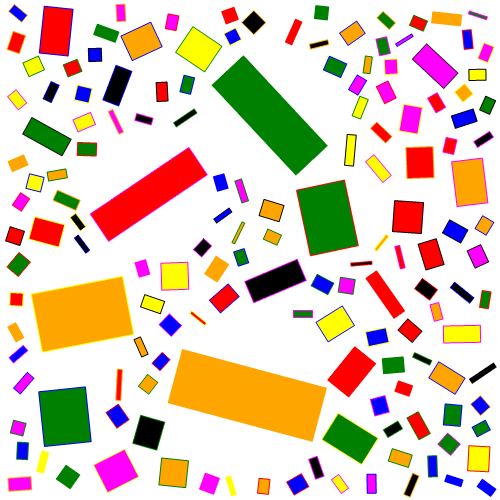
\includegraphics[width=0.60\textwidth]{exmp.png}
\end{center}
}{34
}%
\end{example}

\end{problem}

